\documentclass[review]{elsarticle}

\usepackage{xr} %% For cross-referencing supl figures
\externaldocument[S-]{Supplementary}

\usepackage{lineno,hyperref}
\usepackage[utf8]{inputenc}
\usepackage{graphicx}
\usepackage{amsfonts}
\usepackage{mathtools}
\usepackage{tikz}
\usetikzlibrary{shapes,arrows,chains,calc}

% Set up a few colours for tikz figure
\colorlet{lcfree}{green}
\colorlet{lcnorm}{blue}
\colorlet{lccong}{red}

\modulolinenumbers[1]

\journal{Ecological Modelling}

%%%%%%%%%%%%%%%%%%%%%%%
%% Elsevier bibliography styles
%%%%%%%%%%%%%%%%%%%%%%%
%% To change the style, put a % in front of the second line of the current style and
%% remove the % from the second line of the style you would like to use.
%%%%%%%%%%%%%%%%%%%%%%%

%% Numbered
%\bibliographystyle{model1-num-names}
%% Numbered without titles
%\bibliographystyle{model1a-num-names}
%% Harvard
%%\bibliographystyle{model2-names.bst}\biboptions{authoryear}
%% Vancouver numbered
%\usepackage{numcompress}\bibliographystyle{model3-num-names}
%% Vancouver name/year
%\usepackage{numcompress}\bibliographystyle{model4-names}\biboptions{authoryear}
%% APA style
%%\bibliographystyle{model5-names}\biboptions{authoryear}
%% AMA style
%\usepackage{numcompress}\bibliographystyle{model6-num-names}
%% `Elsevier LaTeX' style
\bibliographystyle{elsarticle-num}
%%%%%%%%%%%%%%%%%%%%%%%

\begin{document}

\begin{frontmatter}
\title{\emph{MixFishSim}: highly resolved spatiotemporal simulations for
	exploring mixed fishery dynamics}

%%\title{A simulation framework for exploring spatiotemporal dynamics in mixed
%%	fisheries}

%% Group authors per affiliation:
\author[1,2]{Paul J. Dolder\corref{c}}
\cortext[c]{Corresponding author}
\ead{paul.dolder@gmit.ie}

\author[1]{Cóilín Minto}
\author[3]{Jean-Marc Guarini}
\author[4]{Jan Jaap Poos}

\address[1]{Galway-Mayo Institute of Technology (GMIT), Dublin Road, Galway,
	Ireland} 
\address[2]{Centre for Environment, Fisheries and Aquaculture Science (Cefas),
	Pakefield Road, Lowestoft, UK}
\address[3]{Université Pierre et Marie Curie, 4 Place Jussieu, 75005 Paris,
	France}
\address[4]{Wageningen Marine Research, Haringkade 1 1976 CP IJmuiden,
	Netherlands}

\begin{abstract}
%\textcolor{gray}{[Guidance: A concise and factual abstract is required. The abstract 
%should state briefly the purpose of the research, the principal results and
%major conclusions. An abstract is often pnresented separately from the article,
%so it must be able to stand alone. For this reason, References should be
%avoided, but if essential, then cite the author(s) and year(s). Also,
%non-standard or uncommon abbreviations should be avoided, but if essential they
%must be defined at their first mention in the abstract itself.  Graphical
%abstract: Although a graphical abstract is optional, its use is encouraged as
%it draws more attention to the online article. The graphical abstract should
%summarize the contents of the article in a concise, pictorial form designed to
%capture the attention of a wide readership. Graphical abstracts should be
%submitted as a separate file in the online submission system. Image size:
%Please provide an image with a minimum of 531 X 1328 pixels (h X w) or
%proportionally more. The image should be readable at a size of 5 x 13 cm using
%a regular screen resolution of 96 dpi.  Preferred file types: TIFF, EPS, PDF or
%MS Office files.] \\}
%
Fishing exploits spatially and temporally hetergenous fish populations, using
species-unselective gear that can result in unintended, unwanted catch of low
quota or protected species. Reducing these unwanted catches is crucial for
biological and economic sustainability of `mixed fisheries' and implementation
of an ecosystem approach to fishing. \\

To implement effective spatial measures to reduce discards a good understanding
of spatiotemporal fishery dynamics is required. However, traditional
scientific advice is limited by a lack of highly resolved knowledge of
population distribution, movement and how fishers interact with different fish
populations. This reflects that data on fish location at high temporal and
spatial resolutions is expensive and difficult to collect and therefore proxies
inferred from either scientific surveys or commercial catch data are often used
to model distributions, often with limited spatial and temporal resolution. \\ 

To understand how resolution impacts mixed fisheries inference, we develop a
highly resolved spatiotemporal simulation model incorporating: i)
delay-difference population dynamics, ii) population movement using Gaussian
Random Fields to simulate patchy, hetergenously distributed populations, and
iii) fishery dynamics for multiple fleet characteristics based on targetting
via correlated random walk movement and learned behaviour. \\ 

We simulate 20 years of exploitation of the fish populations and use the
results from the fishing model to draw inference on the underlying population
structures. We compare this inference to i) a simulated fixed-site sampling
design commonly used for fisheries monitoring purposes, and ii) the true
underlying population structures input to the simulation, to establish the
potential and limitations of fishery-dependent data - an inherently biased
sampling method due to fisher's targeting- to provide a robust picture of
spatiotemporal distributions. Finally, we simulate an area closure based on
areas defined from commercial the known ("real-population") distribution,
commercial catch data and survey data at different temporal and spatial
resolutions and assess their effectiveness on reducing catches of a fish
population. \\

We conclude from our simulations that commercial data, while not unbiased,
provides a useful tool for managing catches in mixed fisheries if applied at
the correct spatiotemporal scale. \\

[333 words]

\end{abstract}

\begin{keyword}
Some\sep keywords \sep here. Max 6 
\MSC[2010] 00-01\sep  99-00
\end{keyword}

\end{frontmatter}

\linenumbers

\section{Introduction}

%\textcolor{gray}{[Guidance:: State the objectives of the work and provide an 
%adequate background, avoiding a detailed literature survey or a summary of the
%results.] \\}
%
Fishers exploit fish populations that are heterogenously distributed in space
and time with verying knowledge of species distributions using
species-unselective fishing gear. Fisheries that catch an assemblage of
species, known as mixed fisheries, when managed by single-species quotas can
end up discarding overquota catch leading to overexploitation of fish
populations. Reducing discarding is crucial to ensure biological and economic
sustainability of fisheries and implementation of an ecosystem approach to
fisheries. As such there is increasing interest in technical solutions such as
gear and spatial closures as ways of avoiding discards.  \\

Use of spatial management as a tool has been proposed as a method to reduce
discards. However, its implementation is hampered by lack of knowledge of fish
and fishery spatiotemporal dynamics and understanding of the scale at which
processes are important for management. Understanding the correct scale for
spatial management is crucial in order to implement measures at a resolution
that ensures effective management\cite{Dunn2016} while minimising economic
impact. For example, a scale that promotes species avoidance for vulnerable or
low quota species while allowing continuance of sustainable fisheries for
available quota species. \\

Ensuring measures are implemented at an appropriate scale has been a challenge
in the past that has led to ineffectual measures with unitended consequences
such as limited impact towards the management objective or increased benthic
impact on previously unexploited areas (e.g. the cod closure in the North
Sea\cite{Rijnsdorp2001,Dinmore2003}). Since then more refined spatial
information has become available through the combination of logbook and Vessel
Monitoring System (VMS) data\cite{Lee2010, Bastardie2010, Gerritsen2012,
	Mateo2016} and more real-time spatial management has been possible 
	(e.g. \cite{Holmes2011}). Such information is, however, patchy and
derived from an inherently biased sampling programme (i.e. targeted fishing).
Further, fishers generally only recorded landings (not catch) on a daily basis.
This leads to questions about the validity of inference that can be drawn from
landings data assigned to VMS activity pings. \\ 

In order to understand challenges that face VMS-linked landings to draw
inference on the underlying population structure we develop a simulation model
where population dynamics are highly-resolved in space and time and are known
rather than inferred from sampling or commercial catches. Population movement
is driven by a random (diffusive) and directed (advective) process and we
incorporate characterisation of a number of different fisheries exploiting four
fish populations with different spatial and population demographics.\\

Using our model we simulate 20 years of exploitation of the fish populations
and use the results from the fishing model to draw inference on the underlying
population structures.  We compare this inference to: i) a stratified
fixed-site sampling survey design commonly used for fisheries monitoring
purposes, otherwise know as a fisheries-independent
	survey, and ii) the underlying population structures input to the
simulation.\\

We simulate a fishery closure to protect one species based on the
fishery-dependent inferred distributions at a spatial and temporal scale
typical in fisheries management, and assess a theoretical "benefit" to the
population, and effect on the other three populations. Further, we extend our
analysis to a range of spatial and temporal scales to assess the impact of
these processes on the success of the management measure. \\

\section{Materials and Methods}

%\textcolor{gray}{[Guidance: Provide sufficient details to allow the work to be
%reproduced by an independent researcher. Methods that are already published
%should be summarized, and indicated by a reference.  If quoting directly from a
%previously published method, use quotation marks and also cite the source. Any
%modifications to existing methods should also be described.] \\ }
%
We develop a simulation model with a modular event-based approach, where
modules are implemented on independent time-scales appropriate to capture the
characteristic of the process modelled (Figure 1). The fishing model operated on a
tow-by-tow basis, while population dynamics (fishing and natural mortality,
growth) operate on a daily time-step.  Population movement occurs on a
weekly time-step, while recruitment occurs periodcally each year for a set
time period (e.g. 3 weeks) at at specified point individual to a species. The
simulation framework is implemented in the statistical software package R
\cite{RCoreTeam2017}; available as an R package from the authors github
(\url{www.github.com/pdolder/MixFishSim}).\\

Here we describe each of the model components; 1)
Population dynamics, 2) Recruitment dynamics, 3) Population movement, 4)
fishery dynamics.

%%%%%%%%%%%%%%%%%%%%%%%%%%%%%%%%%%%
% Overview schematic  
\begin{figure}[!ht]
	\hspace{-4em}
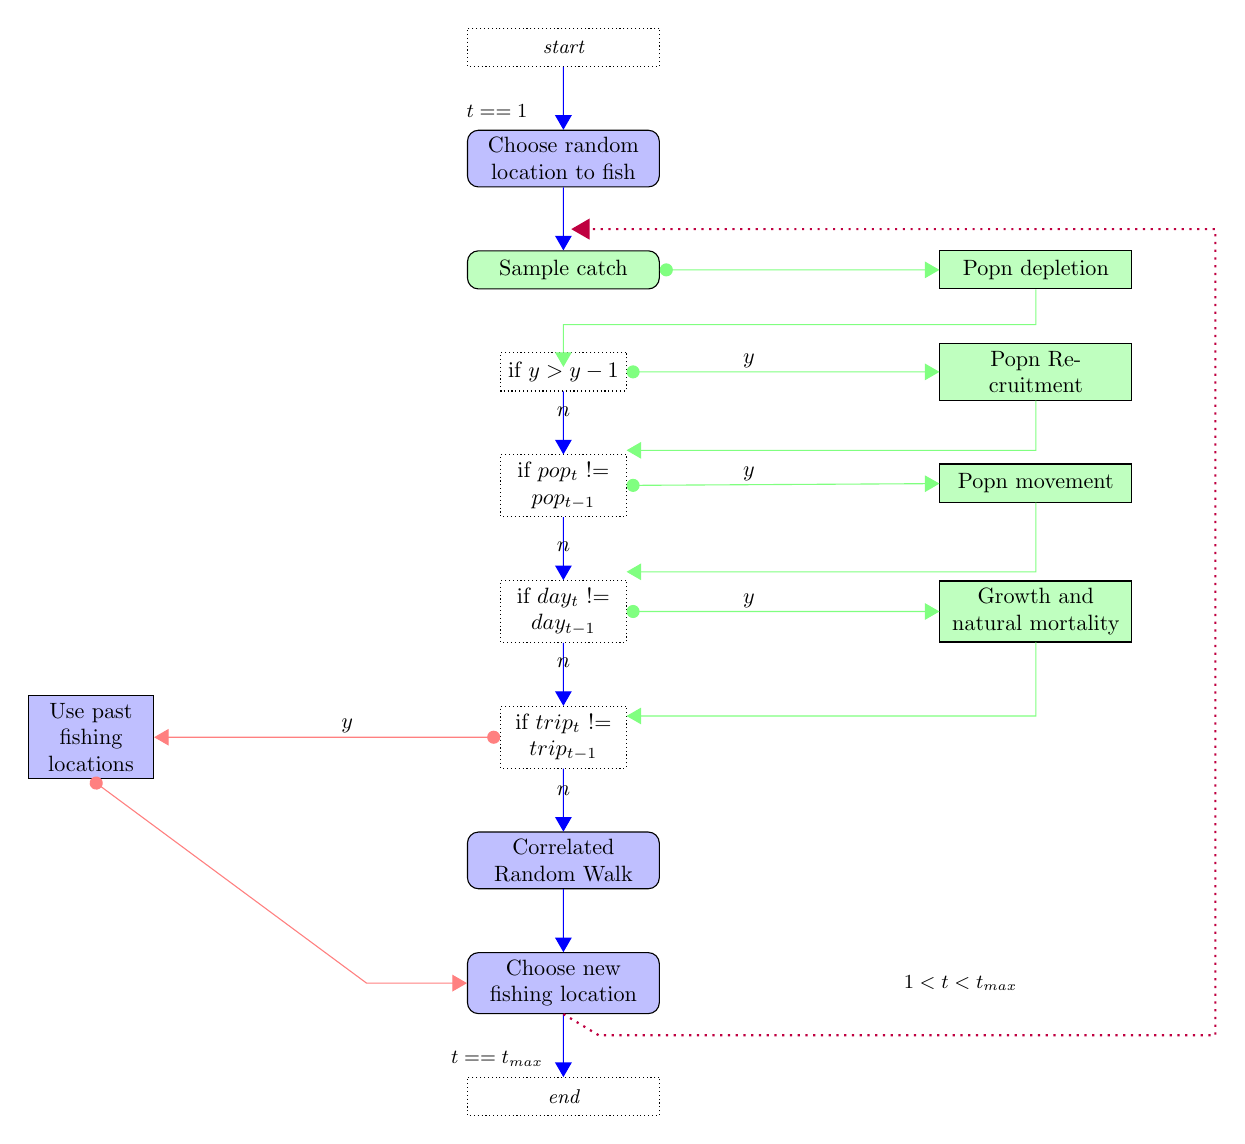
\begin{tikzpicture}[%
    >=triangle 60,              % Nice arrows; your taste may be different
    start chain=going below,    % General flow is top-to-bottom
    node distance=8mm and 60mm, % Global setup of box spacing
    every join/.style={norm},   % Default linetype for connecting boxes
    scale=0.9,
    every node/.style={scale=0.8}]                 
    \label{fig:model}
    % ------------------------------------------------- 
% A few box styles 
% <on chain> *and* <on grid> reduce the need for manual relative
% positioning of nodes
\tikzset{
  base/.style={draw, on chain, on grid, align=center, minimum height=4ex},
  proc/.style={base, rectangle, text width=8em},
  test/.style={base, rectangle, text width=5em},
  term/.style={proc, rounded corners},
  % coord node style is used for placing corners of connecting lines
  coord/.style={coordinate, on chain, on grid, node distance=6mm and 25mm},
  % nmark node style is used for coordinate debugging marks
  nmark/.style={draw, cyan, circle, font={\sffamily\bfseries}},
  % -------------------------------------------------
  % Connector line styles for different parts of the diagram
  norm/.style={->, draw, lcnorm},
  free/.style={->, draw, lcfree},
  cong/.style={->, draw, lccong},
  it/.style={font={\small\itshape}}
}
% -------------------------------------------------
% Start by placing the nodes in the middle
\node [proc, densely dotted, it] (p0) {start};
% Use join to connect a node to the previous one 
\node [term, join, fill=lcnorm!25]      {Choose random location to fish};
\node [term, join, fill=lcfree!25] (p1){Sample catch};
\node [test, densely dotted] (t1) {if $y > y-1$};
\node [test, join, densely dotted] (t2) {if $pop_{t}$ != $pop_{t-1}$};
\node [test, join, densely dotted] (wk) {if $day_{t}$ != $day_{t-1}$};
\node [test, join, densely dotted] (t3) {if $trip_{t}$ != $trip_{t-1}$};
\node [term, join, fill=lcnorm!25]  (p2) {Correlated Random Walk};
\node [term, join, fill=lcnorm!25]  (p3) {Choose new fishing location};
\node [proc, densely dotted, join, it] (p7) {end};

% Right nodes
\node [proc, fill=lcfree!25, right=of p1] (p4) {Popn depletion};
\node [proc, fill=lcfree!25, right=of t1] (p5) {Popn Recruitment};
\node [proc, fill=lcfree!25] (p6) {Popn movement};
\node [proc, fill=lcfree!25, right=of wk] (wk1) {Growth and natural
	mortality};

% left nodes
\node [test, fill=lcnorm!25, left=of t3] (t4) {Use past fishing locations};

% -------------------------------------------------
% A couple of boxes have annotations
\node [below=of p0, it, yshift=1.5em,xshift=-3em] {$t==1$};
\node [right=30mm of p3, it] {$1 < t < t_{max}$};
\node [below=of p3, it,xshift=-3em, yshift=1.5em] {$t == t_{max}$};

% -------------------------------------------------
% First, the straight north-south connections. In each case, we first
% draw a path with a (consistently positioned) annotation node, then
% we draw the arrow itself.
  \draw [*->,lcfree!50] (p1) -- (p4);
\path (t1) to node [near start, xshift=2em, yshift=0.5em] {$y$} (p5); 
  \draw [*->,lcfree!50] (t1) -- (p5);
\path (t2) to node [near start, xshift=2em, yshift=0.5em] {$y$} (p6); 
  \draw [*->,lcfree!50] (t2) -- (p6);
\path (t3) to node [near start, xshift=-3em, yshift=0.5em] {$y$} (t4); 
  \draw [*->,lccong!50] (t3) -- (t4);
\path (wk) to node [near start, xshift=2em, yshift=0.5em] {$y$} (wk1); 
  \draw [*->,lcfree!50] (wk) -- (wk1);

% left to right paths
\path (t1) to node [near start, yshift=-0.2em] {$n$} (t2) ;  
\path (t2) to node [near start, yshift=0.8em] {$n$} (t3) ;  
\path (wk) to node [near start, yshift=-0.2em] {$n$} (t3) ;  
\path (t3) to node [near start, yshift=-0.3em] {$n$} (p2) ;  

% ------------------------------------------------- 
% the twisty connectors. Again, we place the annotation
% first, then draw the connector

\node [coord, left=of p3] (c1)  {};  
\draw [*->,lccong!50] (t4.south) -- (c1) |- (p3);

\node[coord, below=of p4] (c2) {};
\node[coord, above=of t1] (c3) {};
\draw [-<,lcfree!50] (p4.south) -- (c2) |- (c3) |- (t1.north);

\node[coord, below=of p5] (c4) {};
\draw [->,lcfree!50] (p5.south) -- (c4) |- ($(t2.east) + (0,0.5)$);

\node[coord, below=of p6] (c71) {};
\draw [->,lcfree!50] (p6.south) -- (c71) |- ($(wk.east) + (0,0.56)$);

\node[coord, below=of wk1] (c7) {};
\draw [->,lcfree!50] (wk1.south) -- (c7) |- ($(t3.east) + (0,0.3)$);

% -------------------------------------------------
% A last flourish which breaks all the rules
\draw [->,purple, dotted, thick, shorten >=1mm]
  (p3.south) -- ++(5mm,-3mm)  -- ++(87mm,0mm) 
  |- node [black, near end, yshift=1.75em, it]
    {} ($(p1.north) + (0,0.3)$);
% -------------------------------------------------
\end{tikzpicture}
\caption{Overview Schematic of simulation model. The blue boxes indicate fleet
	dynamics processes, the green boxes population dynamics processes while
	the white boxes are the timesteps at which processes occur; $t$ = tow,
	$tmax$ is the total number of tows, $y$ = year, $pop_{t}$ is time of
	population movement, $day$ is a day timestep, $trip$ is a trip time
	step. 
	} 
\label{fig:overview}
\end{figure}
%%%%%%%%%%%%%%%%%%%%%%%%%%

\subsection{Population dynamics}

The basic population level processes are simulated using a modified two-stage
Deriso-Schnute delay difference model \cite{Deriso1980, Schnute1985,
	Dichmont2003} occurring at a daily time-step. Here, population biomass
growth and depletion for pre-recruits and fish recruited to the fishery are
modelled separately as a function of previous recruited biomass, intrinsic
population growth and recruitment:

\begin{equation*}
	\begin{split}
	B_{y,d+1} = &\\
	& (1 + \rho) B_{y,d} \cdot e^{-Z_{y,d}} - \rho \cdot e^{-Z_{y,d}} \hspace{2.9cm}
	\times \\  
	& (B_{y,d-1} \cdot e^{-Z_{y,d-1}} + Wt_{R-1} \cdot \alpha_{d-1} \cdot R_{\tilde{y}(y,d-1)})
	\hspace{0.4cm} + \\
	& Wt_{R} \cdot \alpha_{d} \cdot R_{\tilde{y}(y,d)} 
	\end{split}
\end{equation*}

where $\rho$ is Brody's coefficient, shown to be approximately equal to
$exp(-K)$, where $K$ is the growth rate from a von bertalanffy logistic growth
model \cite{Schnute1985}. $Wt_{R-1}$ is the weight of fish prior to
recruitment, while $Wt_{R}$ is the recruited weight. $\alpha_{d}$ represents
the proportion of fish recruited during that day for the year, while
$R_{\tilde{y}}$ is the annual recruits. \\

Mortality $Z$ can be decomposed to natural mortality, $M$, and fishing
mortality, $F$, where both $M$ and $F$ are instantaneous rates with $M$ fixed
and $F$ calculated by solving the Baranov catch equation \cite{Hilborn1992b}
for $F$:

\begin{equation*}
C_{d} = \frac{F_{d}}{F_{d}+M_{d}} * (1 - e^{-(F_{d} + M_{d})}) * B
\end{equation*}

where $C$ is the summed catch from the fishing model across all fleets and
vessels for the population during the day, and $B$ the daily biomass for the
species. \textcolor{red}{[link $F$ to effort and catchability - as I think we
	have F as an emergent property of the fleets rather than something we
	solve for (I could be wrong though!) - catch for a vessel is a product of
	catchability and biomass, i.e. C = qB, but this catch is summed to
	solve for F. So its both really]}\\

\subsection{Recruitment dynamics}

Recruitment is modelled through a function relating the mature biomass to
recruits at time of recruitment. In \emph{mixfishsim}, it can be modelled
either either as a stochastic Beverton-Holt stock-recruit form
(\cite{Beverton1957}): 

\begin{equation*}
	\begin{split}
	\bar{R} = & \frac{(\alpha * B)}{(\beta + B)} \\
	     R \sim & \log N[(\log(\bar{R}),\log(\sigma^2))]
	\end{split}
\end{equation*}
Where $\alpha$ is the maximum recruitment rate, $\beta$ the spawning stock
biomass (SSB) required to produce half the maximum, $B$ current SSB and
$\sigma^2$ the variability in the recruitment due to stochastic
processes. \\

or a stochastic Ricker form \cite{Ricker1954}

\begin{equation*}
	\begin{split}
	\bar{R} = & B * e^{(\alpha - \beta * B)} \\	
   	     R \sim & \log N[(\log(\bar{R}),\log(\sigma^2))]
	\end{split}
\end{equation*}

where $\alpha$ is the maximum productivity per spawner and $\beta$ the density
dependent reduction in productivity as the SSB increases.

\subsection{Population movement}

To simulate how fish populations might be distributed in space and time, we
employed a Gaussian spatial process to model habitat suitability for each of
the populations, with an advection-diffusion process to control how the
populations moved over time with a moving temperature covariate to capture
temporal dependencies. This was intended to balance realism in population
movement, capturing the main directed and random processes, and practicality of
modelling the population rather than individual fish. \\


For the habitat we define a Gaussian random field process, $\{S(x) : x \in
\mathbb{R}^2\}$, that is a stochastic process where any collection of locations
$x_{1}, \dots, x_{n}$ where for each $x_{i} \in \mathbb{R}^2$, the joint
distribution of $S = \{S(x1),\dots S(x_{n})\}$ is multivariate Gaussian. The
distribution is specified by its \textit{mean function}, $\mu(x) = E[S(x)]$ and
its \textit{covariance function}, $\gamma(x,x') = Cov\{S(x),S(x')\}$
\cite{Diggle2007}.\\

The covariance structure affects the smoothness of the surfaces which the
process generates, and we used the \textit{Matérn} family of covariance
structures, one where the correlation strength weakens the further the distance
apart (i.e. the correlation between $S(x)$ and $S(x')$ decreases as the
distance $u = ||x - x'||$ increases).  The \textit{Matérn} correlation is a
two-parameter family where: \\

\begin{center}
	$\rho(u) = \{2^{\kappa -
		1}\Gamma{\kappa}\}^{-1}(u/\phi)^{\kappa}K_{\kappa}(u/\phi)$
\end{center}
	
$K_{\kappa}(.)$ is a modified Bessel function of order $\kappa$, $\phi >
0$ is a scale parameter with the dimensions of distance, and $\kappa > 0$,
called the order, is a shape parameter which determines the smoothness of the
underlying process. \\

The temperature field is simulated to be on a gradient from a South-Westerly to
North-Easterly direction, with temperature in each cell changing gradually on a
week-by-week basis so that initially high temperature areas cycle to lower
temperatures and low temperature areas vice versa. Each population is assigned
a thermal tolerance with mean, $\mu$ and variance, $\sigma^2$ so that each cell
and population temperature suitability is defined that:

\begin{equation}
	Tol_{c, p} = \frac{1}{ \sqrt (2\pi \cdot \sigma^2_{p})} \cdot \exp(-
		\frac{(T_{c} -
		\mu_{p})^2}{2 \cdot \sigma^2_{p}} )	
\end{equation}

Where $Tol_{c,p}$ is the tolerance of population $p$ in cell $c$, $T_{c}$ is
the temperature in the cell and $\mu$ and $\sigma^2$ the mean and standard
deviation of the population temperature tolerance. \\

In the simulation model, the habitat for each of the populations is generated
through the \textit{RFSimulate} function of the \textit{RandomFields} R package
\cite{Schlater2015}, implementing different parameter settings to affect the
patchiness of the populations. Each population is initialised at a single
location, and subsequently moves according to a probabilistic distribtion based
on habitat suitability, temperature and distance from current cell. 

\begin{equation}
	Pr(B | A) = \frac{e^{-\lambda * d_{AB}} \cdot
		(Hab_{B}^2 \cdot Tol_{B,wk})}{\sum\limits_{c=1}^{C}e^{-\lambda * d} \cdot
		(Hab_{B}^2 \cdot Tol_{B,wk})}
\end{equation}

Where $d_{AB}$ is the euclidean distance between cell $A$ and cell $B$,
$\lambda$ is a given rate of decay, $Hab_{B}^2$ is the squared index of habitat
suitability for cell $B$ and $Tol_{B,wk}$ the temperature tolerance for the
cell in week $wk$; population index, $p$ has been dropped for simplicity.\\

During specified weeks of the year, the habitat quality is modified for
spawning habitats, meaning each population has a concentrated area where
spawning takes place and the population moves towards this in the weeks prior
to spawning. \\

\subsection{Fleet dynamics}

The fleet dynamics can be broadly categorised into three components; fleet
targeting - which determines the fleet catch efficiency and preference towards
a particular species; trip-level decisions, which determine the initial
location to be fished at the beginning of a trip; and within-trip decisions,
determining movement from one fishing spot to another within a trip.

\subsubsection{Fleet targeting}

Each fleet of \textit{n} vessels is characterised by both a general efficiency,
\textit{Q}, and a population specific efficiency, ${Q_{p}}$.  Thus, the product
of these parameters affects the overall catch rates for the fleet and the
preferential targeting of one population over another. This, in combination
with the parameter choice for the step-function (as well as some randomness
from the exploratory fishing process) determines the preference of fishing
locations for the fleet.  All species prices are kept the same, across fleets,
though can be made to vary seasonally.  

\subsubsection{Trip-level decisions}

Several studies (e.g.\cite{Hutton2004, Tidd2012, Girardin2015}) have confirmed
past activity and past catch rates are strong predictors of fishing location
choice. For this reason, the fleet dynamics sub-model includes a learning
component, where a vessel's initial fishing location in a trip is based on
selecting from previously successful fishing locations. This is achieved by
sorting all previous fishing events in the previous trip as well as the
previous time periods in past years, and choosing randomly from the top x \% of
fishing events in value.  Simulation testing indicated that this learning
increased the mean value of catches for the vessels, over just relying on the
correlated random walk function. 

\subsubsection{Within-trip decisions}

Fishing locations within a trip are determined by a modified random walk
process. A random walk type was chosen as it is the simplest assumption
commonly used in ecology to describe animal movement which searching for
homogeneously distributed prey about which there is uncertain knowledge. In a
random walk, movement is a stochastic process through a series of steps that
can either be equal in length or take some other functional form.  The
direction of the random walk can be correlated, a characteristic known as
`persistence', providing some overall location of directional movement
\cite{Codling2008} or uncorrelated. \\

A \textit{lévy walk} is a particular form of random walk characterised by a
heavy-tailed distribution of step-length and has received a lot of attention in
ecological theory in recent years as having shown to have very similar
characteristics as those observed by animals in nature, and being a near
optimum searching strategy for predators pursuing patchily distributed prey
\cite{Bartumeus2005, Sims2008}.  \cite{Bertrand2007} showed that Peruvian
anchovy fishermen have a stochastic search pattern similar to that observed
with a lévy walk. However, it remains a subject of debate, with the contention
that search patterns may be more simply characteristed as random walks
\cite{Sakiyama2013} with specific patterns related to the characteristics of
the prey field \cite{Sims2012}. \\

We use a modified random walk where directional change is based on a correlated
circular distribution where a favourable fishing ground is likely to be ``fished
back over" by the vessel returning in the direction it came from and step
length (i.e. the distance travelled from the current to the next fishing
location) is determined by relating recent fishing success, measured as the
summed value of fish caught, $$Rev = \sum_{s=1}^{\infty} C_{s} \cdot Pr_{s}$$
where $C_{s}$ is catch of a species, and $Pr_{s}$ price of a species, to step
distance. Here, when fishing is successful vessels remain in a similar location
and continue to exploit the local fishing grounds. When unsuccessful, they move
some distance away from the current fishing location. The movement distance
retains some degree of stochasticity, which can be controlled separately. 

The step function takes the form:

\begin{equation*}
	StepL = e^{log(\beta_{1}) + log(\beta_{2}) - (log(\frac{\beta_{1}}{\beta_{3}}))} * Rev
\end{equation*}

So that, a step from (x1,y1) to (x2, y2) is defined by:

\begin{equation*}
	\begin{split}
 (x2, y2) =  & x1 + StepL \cdot \cos (\frac{\pi \cdot Br}{180}), \\
             & y1 + StepL \cdot \sin (\frac{\pi \cdot Br}{180}) \\	
 with  \hspace{0.5cm}     & Br_{t-1} < 180, Br_{t} = 180 + \sim vm[(0,360), k] \\
 			  & Br_{t-1} > 180, Br_{t} = 180 - \sim vm[(0,360), k] \\
	\end{split}
\end{equation*}

with $k$ the concentration parameter from the von mises distribution which we
correlate with the revenue so that $k = (Rev + 1 / RefRev) * max_{k}$,
where $max_{k}$ is the maximum concentration value, $k$, and RefRev is
parameterised as for $\beta_{3}$ in the step length function. 

\subsubsection{Local population depletion}

Where several fishing vessels are exploiting the same fish population
competition is known to play an important role in local distribution of fishing
effort \cite{Gillis1998}. If several vessels are fishing on the same patch of
fish, local depletion and interference will affect fishing location choice of
the fleet as a whole \cite{Rijnsdorp2000, Poos2007a}. In order to account for
this behaviour, the fishing sub-model operates spatially on a daily time-step
so that for future days the biomass available to the fishery is reduced in the
areas fished. The cumulative effect is to make heavily fished areas less
attractive as future fishing opportunities. 

\subsection{Fisheries independent survey}

A fisheries-independent survey is simulated where fishing on a regular grid
begins each year at the same time for a given number of stations (a fixed
station survey design). Catches of the populations present are recorded but not
removed from the population. This provides a fishery independent snapshot of
the populations at a regular spatial distribution each year, similar to
scientific surveys undertaken by fisheries research agencies. 

\section{Calculation}

%\textcolor{gray}{[Guidance: A \underline{Theory} section should extend, not
%repeat, the background to the article already dealt with in the	Introduction
%and lay the foundation for further work.  In contrast, a
%\underline{Calculation} section represents a practical development from a
%theoretical basis.] \\}
%
\subsection{Population parameterisation}

We parameterised the simulation model for four populations with differing
habitat preference and temperature tolerances (Figures \ref{S-fig:1},
\ref{S-fig:3}, \ref{S-fig:4}, \ref{S-fig:5}, \ref{S-fig:6}, \ref{S-fig:7}),
population demographic and recruitment functions. In addition, each of the
populations has two defined spawning areas which result in the populations
moving towards these areas in given weeks (Figure \ref{S-fig:2}) and
population-specific movement rates (Table \ref{tab:1}). The realised movement
of the populations for a number of weeks is shown in Figure \ref{S-fig:9} while
the realised daily fishing mortality are shown in Figure \ref{S-fig:10}. \\

\subsection{Fleet parameterisation}

The fleets were parameterised to reflect five different characteristics based
on targeting preference and exploitation dynamics (Table \ref{tab:2}). This
ensures that different fleets have different spatial dynamics, preferentially
targeted different fish populations. The stochasticity in the random walk
process ensures that different vessels within a fleet have slightly different
spatial distributions based on individual experience, while the step function
was parameterised dynamically so that vessels take smaller steps where the
fishing location yields in a top quartile of the value available in that year
(as defined per fleet in Table \ref{tab:2}). \\

Each fleet was set so that, after the first year, fishing locations were chosen
based on experience built up in the same month from previous years and from
past trip fishing success. 'Success' in this context was defined as the
locations where the top 75 \% of revenue from was found in previous trips.

An example of the realised fleet movements for a single vessel during a single
trip are given in Figure \ref{S-fig:11}, while Figure \ref{S-fig:12} shows
multiple trips for a single vessel, \ref{S-fig:13} the vessel movements for
some trips overlaid on the value field, \ref{S-fig:14} shows fishing locations
for an entire fleet of 20 vessels for a single trip, while \ref{S-fig:15} shows
an example of the step function realisation and turning angles from the
correlated random walk.

\subsection{Survey settings}

The survey simulation was set up with follow a fixed gridded station design
with 100 stations fished each year, starting on day 92 with same catchability
parameters for all populations (Q = 1). 

\subsection{Simulation settings}

To illustrate the capabilities on \emph{MixFishSim}, we investigate the
influence of the temporal and spatial resolution of different data sources on
the reduction in catches of a population given spatial closures. To do so, we
first set up with simulation to run for 10 years based on a 100 X 100 square
grid, with five fleets of 20 vessels each and four fish populations. Fishing
takes place four times a day per vessel and five days a week, while population
movement is every week. \\

We allow the simulation to run unrestricted for 5 years, and subsequently close
areas for the last 5 years of the simulation based on data (either derived from
the commercial catches, fisheries-independent survey or the 'real population' -
the underlying populations assumed to be known perfectly) used at different
spatial and temporal scales. \\

The following steps are undertaken to determine closures:

\begin{enumerate}
	\item Extract data source
	\item Aggregate according to resolution
	\item Interpolate across entire area at desired resoltion
	\item Close top 5 \% of areas
\end{enumerate}

In total 56 closure scenarios were run which represent combinations of

\begin{itemize}
	\item \textbf{data types:} commercial logbook data, survey data and
		'real population',
	\item \textbf{temporal resolutions:} weekly, monthly and yearly
		closures,
	\item \textbf{spatial resolutions:} 1 x 1 grid, 5 x 5 grid, 10 x 10
		grid and 20 x 20 grid.
\end{itemize}

Survey closures were on an annual basis only, as this was the most temporally
resolved survey data available.

\section{Results}

The species distribution themselves 

The consequences of different spatial aggregations of the data are shown in
Figure \ref{fig:1}, which represents the aggregation of catch from each of the
data sources over a year at different spatial resolutions. \\

The finer spatial grid for the the real population (top left) and commercial
data (top middle) show similar patterns, though there are unsampled gaps in the
commercial data from a lack of fishing activity (particularly in the lower left
part of the sampling domain). The survey data at this spatial resolution shows
very sparse and uninformative information about the spatial distributions of
the populations. The slightly aggregated data on a 5 x 5 grid shows similar
patterns, and while losing some of the spatial detail there remains good
consistency between the 'real population' and the commercial data. Survey data
starts to pick out some of the similar patterns as the other data sources, but
lacks coverage. The spatial catch information on a 10 x 10 and 20 x 20 grid
loses a significant amount of information about the spatial resolutions for all
data sources, and some differences between the commercial and 'real population'
data emerge. \\

Figure \ref{fig:2} shows the consequences of different temporal aggregations of
the data, with 156 weekly (top), 36 monthly (middle) and 3 yearly (bottom)
catch compositions across a 20 x 20 area. \\

As can be seen from the 'real population', the monthly aggregation captures the
major patterns seen in the weekly data, albeit missing more subtle differences.
The yearly data results in a constant catch pattern due to the aggregation
process (sometimes known as an aggregation bias). The commercial data on a
weekly basis shows some of the same patterns as the 'real population', though
the first species (in red) is less well represented and some weeks are missing
catches from the area. The monthly data. The monthly data shows some
consistency between the 'real population' and commercial data for species 2 -
4, though species 1 remains underrepresented. On an annual basis, interestingly
the commercial data underrepresents the first species (in red) while the survey
overrepresents species 1. This is likely due to the biases in commercial
sampling, with the fisheries not targeting the areas where species 1 are
present, and the biases in the survey sampling from overrepresentation of the
spatial distribution. \\

We implemented a spatial closure using the different data sources and spatial
and temporal aggregations as outlined in the protocol in Section 3.4. We used
this to assess the efficacy of a closure in reducing fishing mortality on
species 1, given availability of data and its use at different resolutions in
order to evaluate the trade-offs in data sources. Figure \ref{fig:3} shows the
trend in fishing mortality for each species simulated (columns) given the data
sources (rows), temporal aggregations (colour lines) and spatial aggregations
(linestyles), while Figure \ref{fig:4} shows the change in fishing mortality
from before the closure (average F years 2 - 4) to after the closure (average F
years 8 - 10). \\

For the closures based on 'real population' (bottom row), the most
disaggregated data (a weekly timescale and 1 x 1 resolution) was most
effective, reducing fishing mortality on species 1 (left) by $\sim$ 60 \%. Next
was the monthly closures ($<$ $\sim$ 30 \%).  The least effective were the
yearly closures (blue lines) at all spatial resolutions, which resulted in
increased fishing mortalities ($>$ 30 \% - \textcolor{blue}{N.B. Note though,
this is consistent with the increasing trends in F, which is probably more
related to the fact that Fs hadn't stabilised in the simulation from the
fishing vessels "learning" the best locations - I will rerun the sims for a
longer time (20 - 30 years)}. \\

For the survey data, which can only be implemented on a yearly timescale, the
closures had no effect at any data resolution. The results are identical for
the different data resolutions except 20 x 20, which is why you can't see more
than 2 points. This is because of the sparsity of the sampling locations.\\

For the commercial data, the most effective closure scenario was based on 1 x 1
data at a monthly temporal resolution. This results in $\sim$ 10 \% reduction
in F for species 1. \textcolor{blue}{This was the only closure scenario to have
	positive effect according to Figure \ref{fig:4}, though looking at the
	trend in Figure \ref{fig:3} this looks more related to the continued
	increased in F trend, as other scenarios had an initial effect}.
Interestingly the monthly data scenario was more effective than weekly data,
which I'd posit is due to the increase amount of data available from the
commercial sampling across a month compared to a week.i Commercial data used at
an annual timestep was ineffective in bringing fishing mortality down for
species 1. \\

Given the scenarios above, it seems clear that spatial disaggregation is more
important than the temporal disaggregation of the commercial data, except when
its used at an annual timeframe, which is the scenario that gave the worst
results.

For the other species in the simulation (population 2 - 4) there was little
difference in fishing mortalities across scenarios.

\textcolor{blue}{Note: The monthly commercial data scenario is the most
	effective of the realistic scenarios, as the 'real population' can only
	be seen as a baseline comparison.}


%\textcolor{gray}{[Guidance: Results should be clear and concise.]}

\section{Discussion}

%\textcolor{gray}{[Guidance: This should explore the significance of the results 
%of the work, not repeat them. A combined Results and Discussion section is
%often appropriate.  Avoid extensive citations and discussion of published
%literature.]}
%
\section{Conclusions}

%\textcolor{gray}{[Guidance: The main conclusions of the study may be presented 
%in a short Conclusions section, which may stand alone or form a subsection of a
%Discussion or Results and Discussion section.]}
%
\section*{Appendices}

%\textcolor{gray}{[Guidance: If there is more than one appendix, they should 
%be identified as A, B, etc.  Formulae and equations in appendices should be
%given separate numbering: Eq.  (A.1), Eq. (A.2), etc.; in a subsequent
%appendix, Eq. (B.1) and so on.  Similarly for tables and figures: Table A.1;
%Fig. A.1, etc.]}
%
\begin{table}[!ht]
\caption{Population dynamics and movement parameter setting}
	\begin{tabular}{ p{4cm } p{2cm} p{2cm} p{2cm} p{2cm}}
	Parameter & Pop 1 & Pop 2 & Pop 3 & Pop 4 \\
	\hline
	Habitat quality & & & \\
	\hline
	Matérn $\nu$ & 1/0.15 & 1/0.05 & 1/0.55 & 1/0.05  \\
	Matérn $\kappa$ & 1 & 2 & 1 & 1  \\
	Anisotropy & 1.5,3,-3,4 & 1,2,-1,2 & 2.5,1,-1,2 & 0.1,2,-1,0.2 \\
	Spawning areas (bound box) & 40,50,40,50; 80,90,60,70 &
	50,60,30,40; 80,90,90,90 & 30,34,10,20; 60,70,20,30 & 50,55,80,85; 30,40,30,40 \\
	Spawning multiplier & 10 & 10 & 10 & 10 \\
	Movement $\lambda$ & 0.3 & 0.3 & 0.3 & 0.3 \\
	\hline
	Population dynamics & & & & \\
	\hline
	Starting Biomass & 1e5 & 2e5 & 1e5 & 1e4 \\
	Beverton-Holt Recruit 'a' & 60 & 100 & 80 & 2 \\
	Beverton-Holt Recruit 'b' & 250 & 250 & 200 & 50 \\
	Beverton-Holt Recruit $\sigma^2$ & 0.4 & 0.3 & 0.4 & 0.3 \\
	Recruit week & 13-16 & 12-16 & 14-16 & 16-20 \\
	Spawn week & 16-18 & 16-19 & 16-18 & 18-20 \\
	$K$ & 0.3 & 0.3 & 0.3 & 0.3 \\
	$wt$ & 1 & 1 & 1 & 1 \\
	$wt_{d-1}$ & 0.1 & 0.1 & 0.1 & 0.1 \\
	M (annual) & 0.2 & 0.2 & 0.2 & 0.1 \\
	\hline
\end{tabular}
\label{tab:1}
\end{table}

\begin{table}[!ht]
\caption{Fleet dynamics parameter setting}
\begin{tabular}{ p{4cm } p{1cm} p{1cm} p{1cm} p{1cm} p{1cm}}
	\hline
	Parameter & Fleet 1 & Fleet 2 & Fleet 3 & Fleet 4 & Fleet 5 \\
	\hline
	Targeting preferences &&&& \\
	\hline
	Price Pop1 & 100 & 100 & 100 & 100 & 100 \\
	Price Pop2 & 200 & 200 & 200 & 200 & 200 \\
	Price Pop3 & 600 & 600 & 600 & 600 & 600 \\
	Price Pop4 & 1600 & 1600 & 1600 & 1600 & 1600 \\
	$Q$ Pop1 & 0.01 & 0.02 & 0.02 & 0.01 & 0.01 \\
	$Q$ Pop2 & 0.02 & 0.01 & 0.02 & 0.01 & 0.03\\
	$Q$ Pop3 & 0.01 & 0.02 & 0.02 & 0.01 & 0.02 \\
	$Q$ Pop4 & 0.02 & 0.01 & 0.02 & 0.05 & 0.01 \\
	\hline
	Exploitation dynamics &&&& \\
	\hline
	step function $\beta_1$ & 1 & 2 & 1 & 2 & 3 \\
	step function $\beta_2$ & 10 & 10 & 8 & 12 & 7 \\
	step function $\beta_3$ & Q90 & Q90 & Q85 & Q90 & Q80 \\
	step function $rate$ & 10 & 20 & 15 & 25 & 10 \\
	Past Knowledge & T & T & T & T & T \\
	Past Year \& Month & T & T & T & T & T \\
	Past Trip & T & T & T & T & T \\
	Threshold & 0.75 & 0.75 & 0.75 & 0.75 & 0.75 \\
	\hline
\end{tabular}
\label{tab:2}
\end{table}

\begin{figure}[!ht]
	\includegraphics[width =\linewidth]{../analysis/Data_Aggregation_space}
	\caption{Data aggregation at different spatial resolutions}
	\label{fig:1}
\end{figure}	

\begin{figure}[!ht]
	\includegraphics[width = \linewidth]{../analysis/Data_Aggregation_time}
	\caption{Data aggregation at different temporal resolutions}
	\label{fig:2}
\end{figure}	


\begin{figure}[!ht]
	\includegraphics[width = \linewidth]{../analysis/F_trends}
	\caption{Comparison of closure scenarios - F trends}
	\label{fig:3}
\end{figure}	

\begin{figure}[!ht]
	\includegraphics[width = \linewidth]{../analysis/Overview_plot_highPop}
	\caption{Comparison of closure scenarios}
	\label{fig:4}
\end{figure}	

\section*{Abbreviations} Detail any unusual ones used.

\section*{Acknowledgements} those providing help during the research..

\section*{Funding} This work was supported by the MARES doctoral training
program; and the Centre for Environment, Fisheries and Aquaculture Science
seedcorn program.

\clearpage

\section*{References}

\bibliography{simulation_framework}

\end{document}
